\documentclass{beamer}
\special{landscape}

%\usetheme{Berlin}
\usetheme{Warsaw}

%\usecolortheme{seahorse}
%\usefonttheme[onlysmall]{structurebold}

\setbeamertemplate{headline}[split]
\setbeamertemplate{footline}[default]
\setbeamertemplate{footline}[miniframes theme]
%\logo{\includegraphics[scale=0.25]{lifia_logo.png}}

\mode<presentation>
\usepackage[spanish]{babel}
\usepackage{beamerthemesplit}
\usepackage[utf8]{inputenc}
\usepackage{color}      % use if color is used in text


% Comandos en modo Verbatim
%\usepackage{fancyvrb}


\title{Practica 1 - Subrutinas}
%\author{Juan Antonio Zubimendi\\azubimendi@lifia.info.unlp.edu.ar}

%\institute{LINSE}
%\date{24/04/2008}

\AtBeginSection[]

\begin{document}

\begin{frame}
%\frametitle{Presentación}
\titlepage
\end{frame}

\section{Introducion}

\begin{frame}
\frametitle{Ejercicio 7 - Pasaje de parámetros por pila}
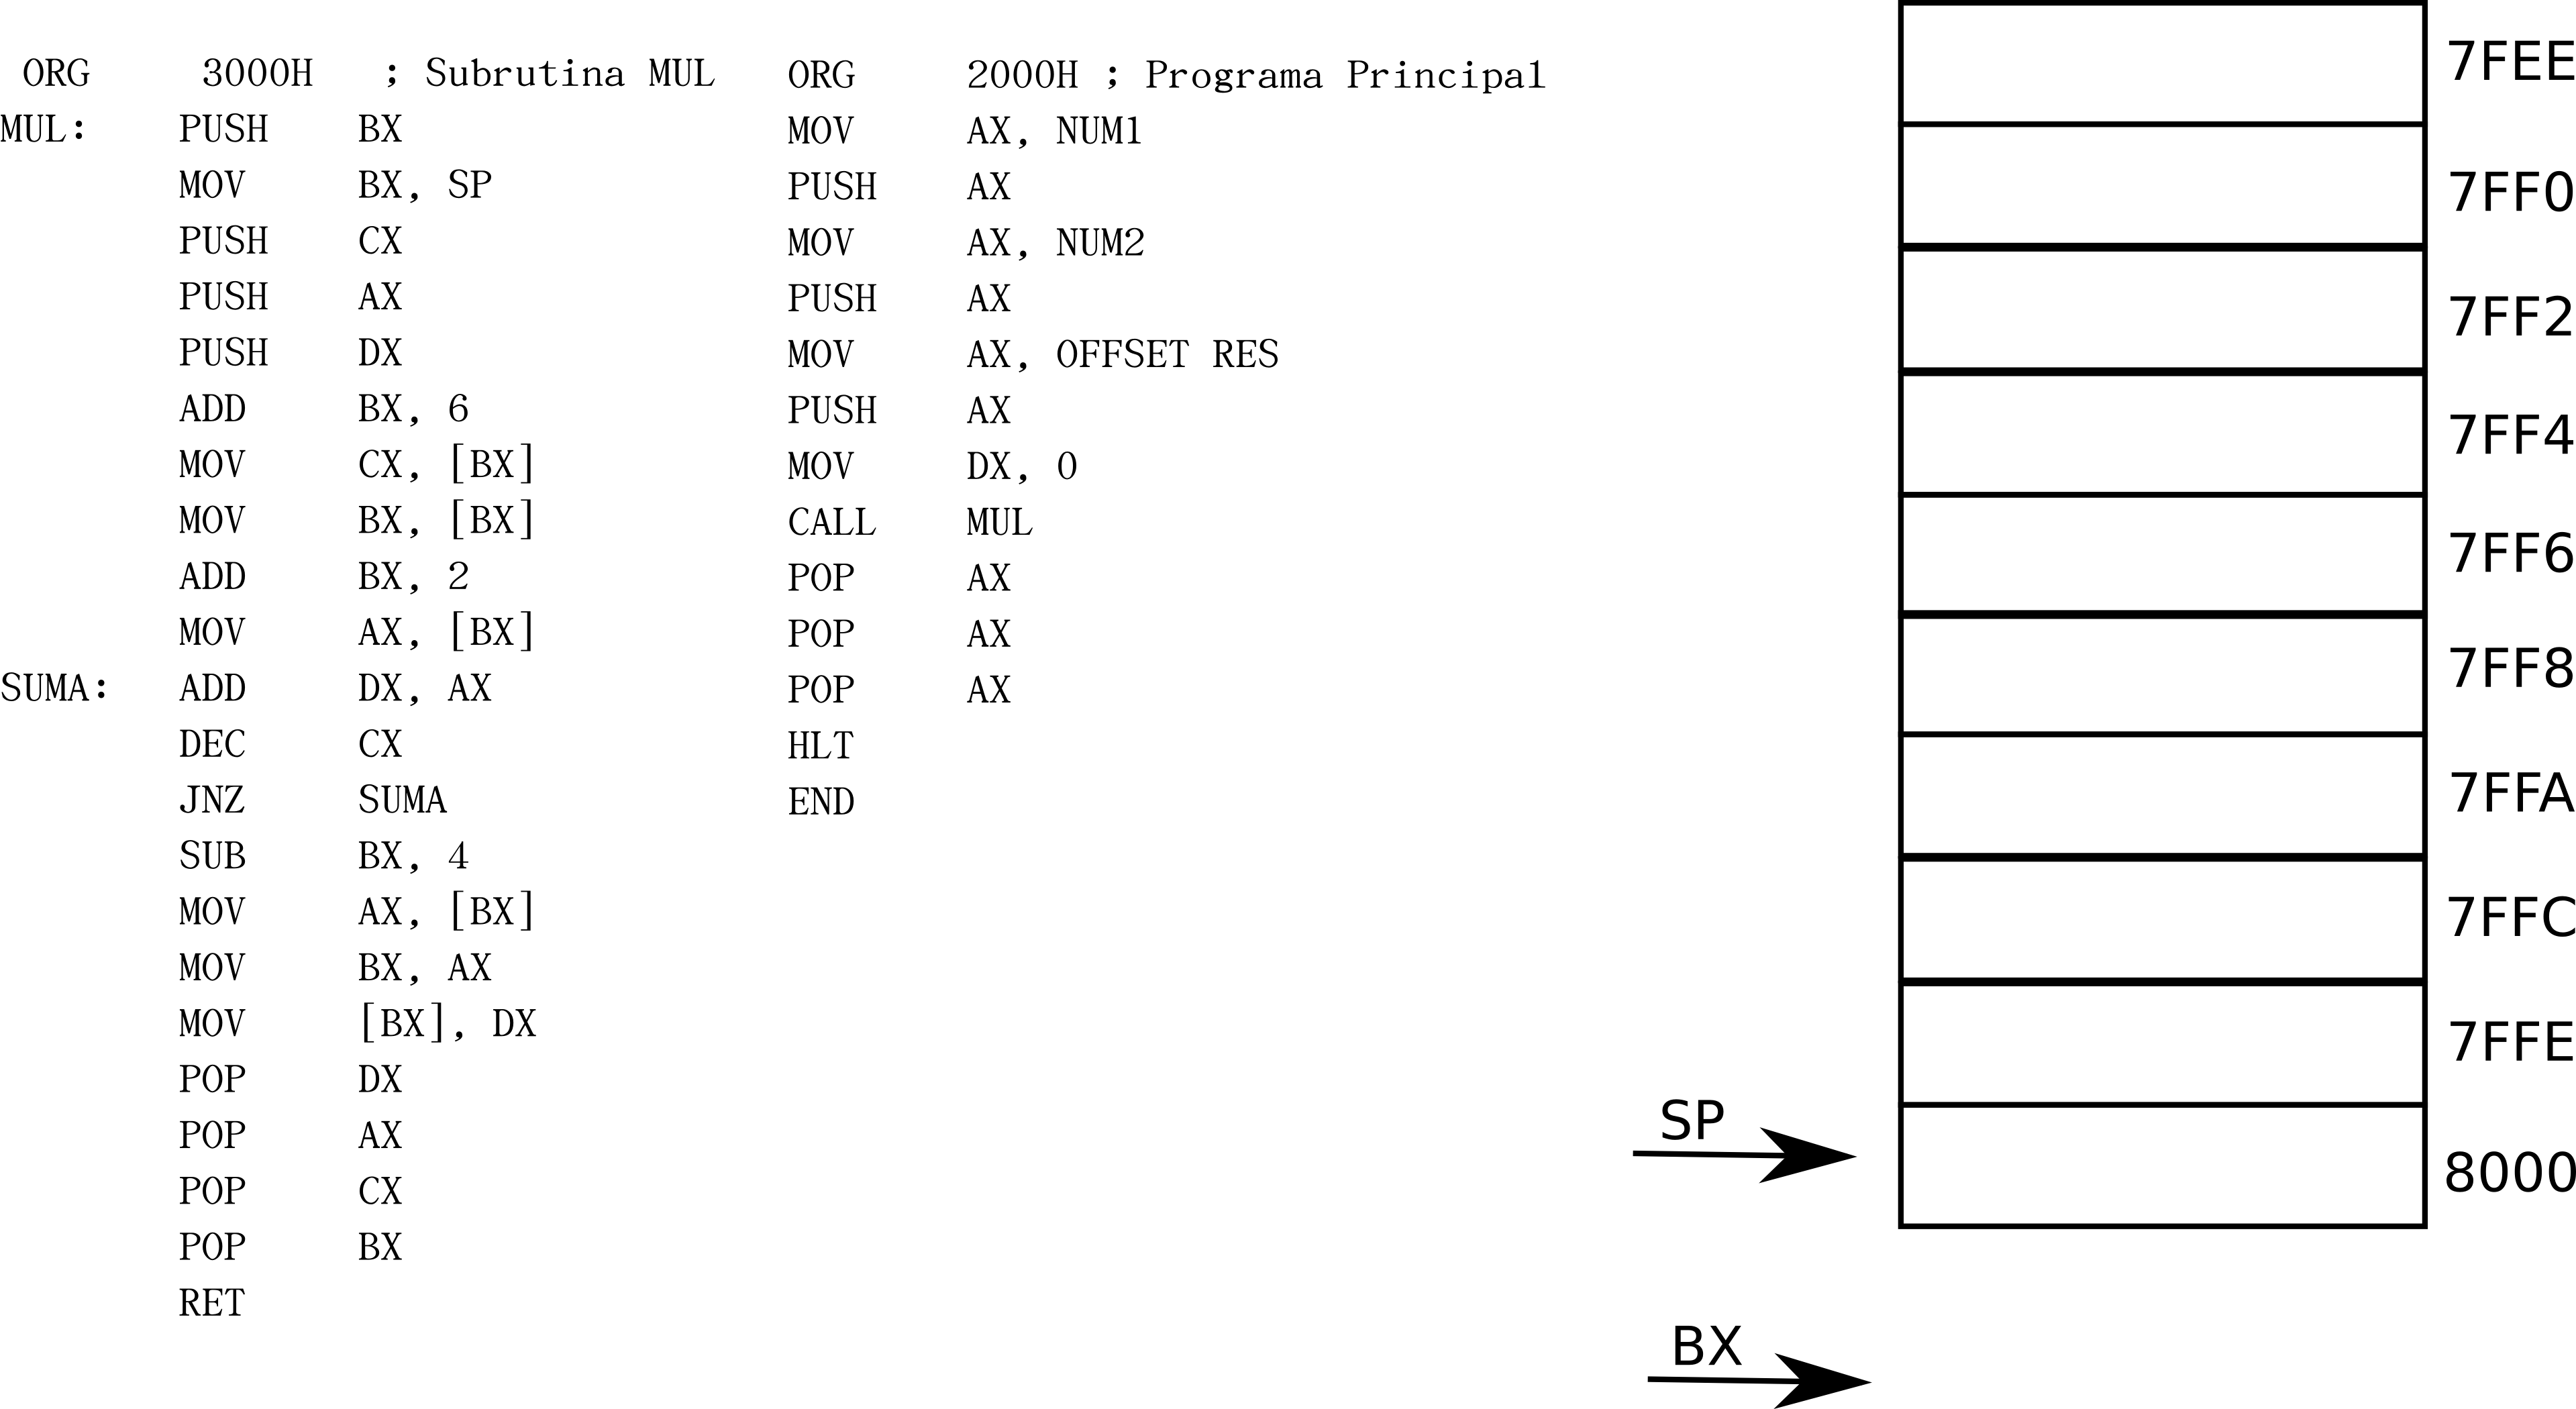
\includegraphics[scale=0.70]{imgs/imagen_001.png}
\end{frame}

\begin{frame}
\frametitle{Ejercicio 7 - Pasaje de parámetros por pila}
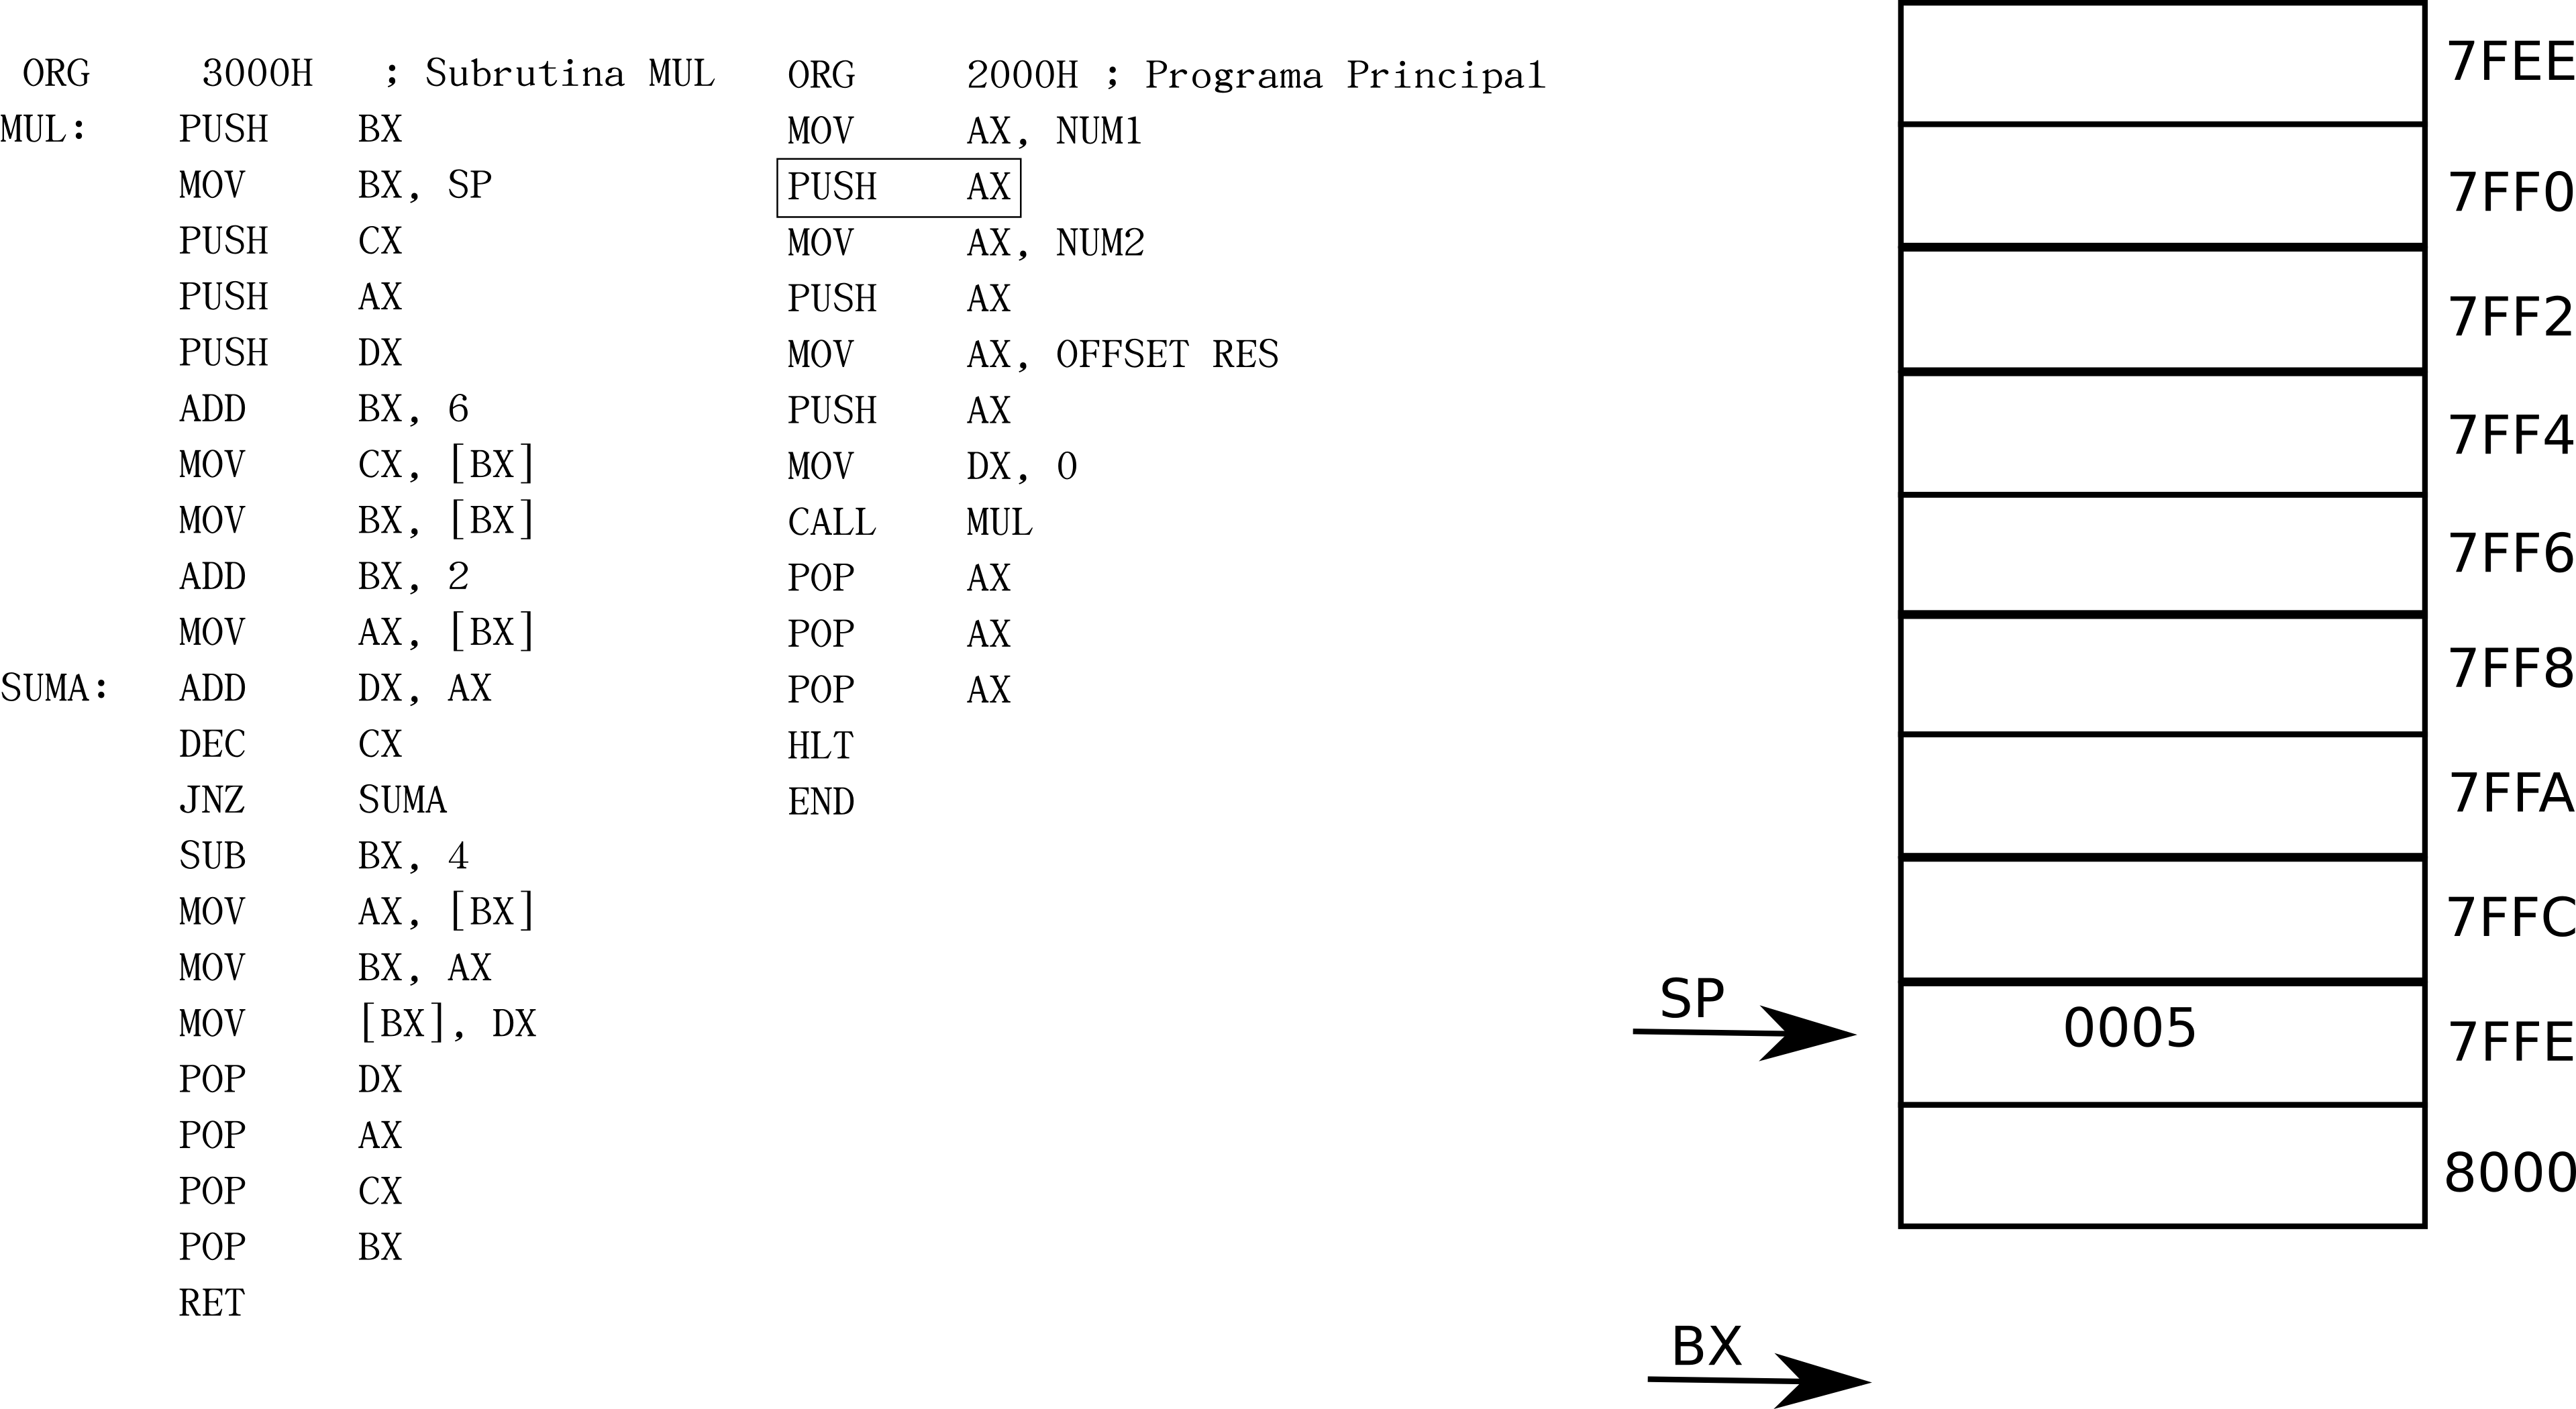
\includegraphics[scale=0.70]{imgs/imagen_002.png}
\end{frame}

\begin{frame}
\frametitle{Ejercicio 7 - Pasaje de parámetros por pila}
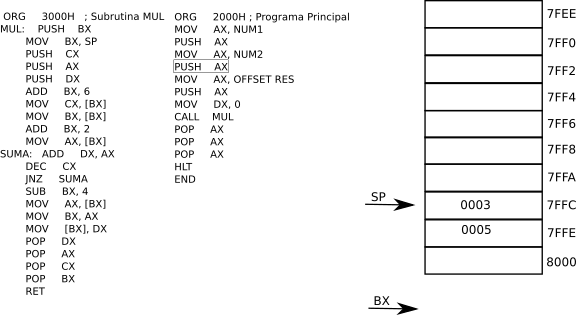
\includegraphics[scale=0.70]{imgs/imagen_003.png}
\end{frame}

\begin{frame}
\frametitle{Ejercicio 7 - Pasaje de parámetros por pila}
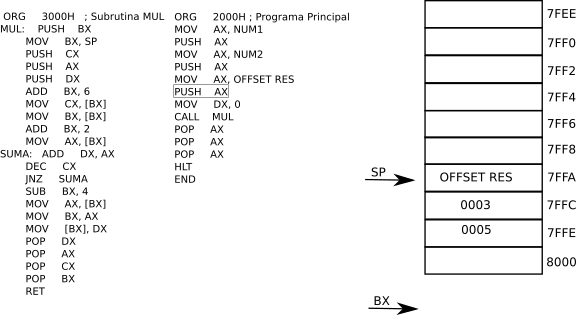
\includegraphics[scale=0.70]{imgs/imagen_004.png}
\end{frame}

\begin{frame}
\frametitle{Ejercicio 7 - Pasaje de parámetros por pila}
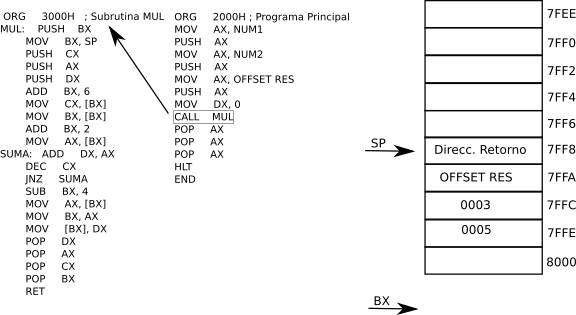
\includegraphics[scale=0.70]{imgs/imagen_005.png}
\end{frame}

\begin{frame}
\frametitle{Ejercicio 7 - Pasaje de parámetros por pila}
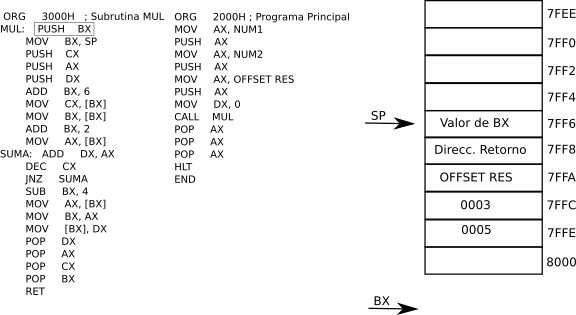
\includegraphics[scale=0.70]{imgs/imagen_006.png}
\end{frame}
\begin{frame}
\frametitle{Ejercicio 7 - Pasaje de parámetros por pila}
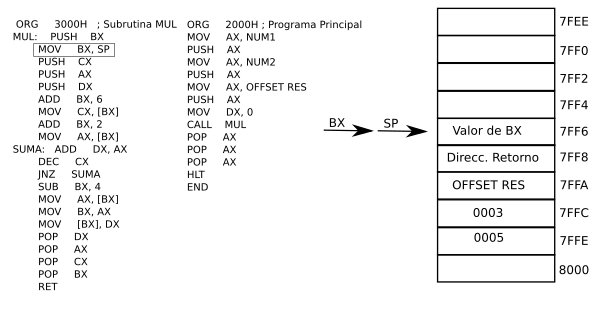
\includegraphics[scale=0.70]{imgs/imagen_007.png}
\end{frame}
\begin{frame}
\frametitle{Ejercicio 7 - Pasaje de parámetros por pila}
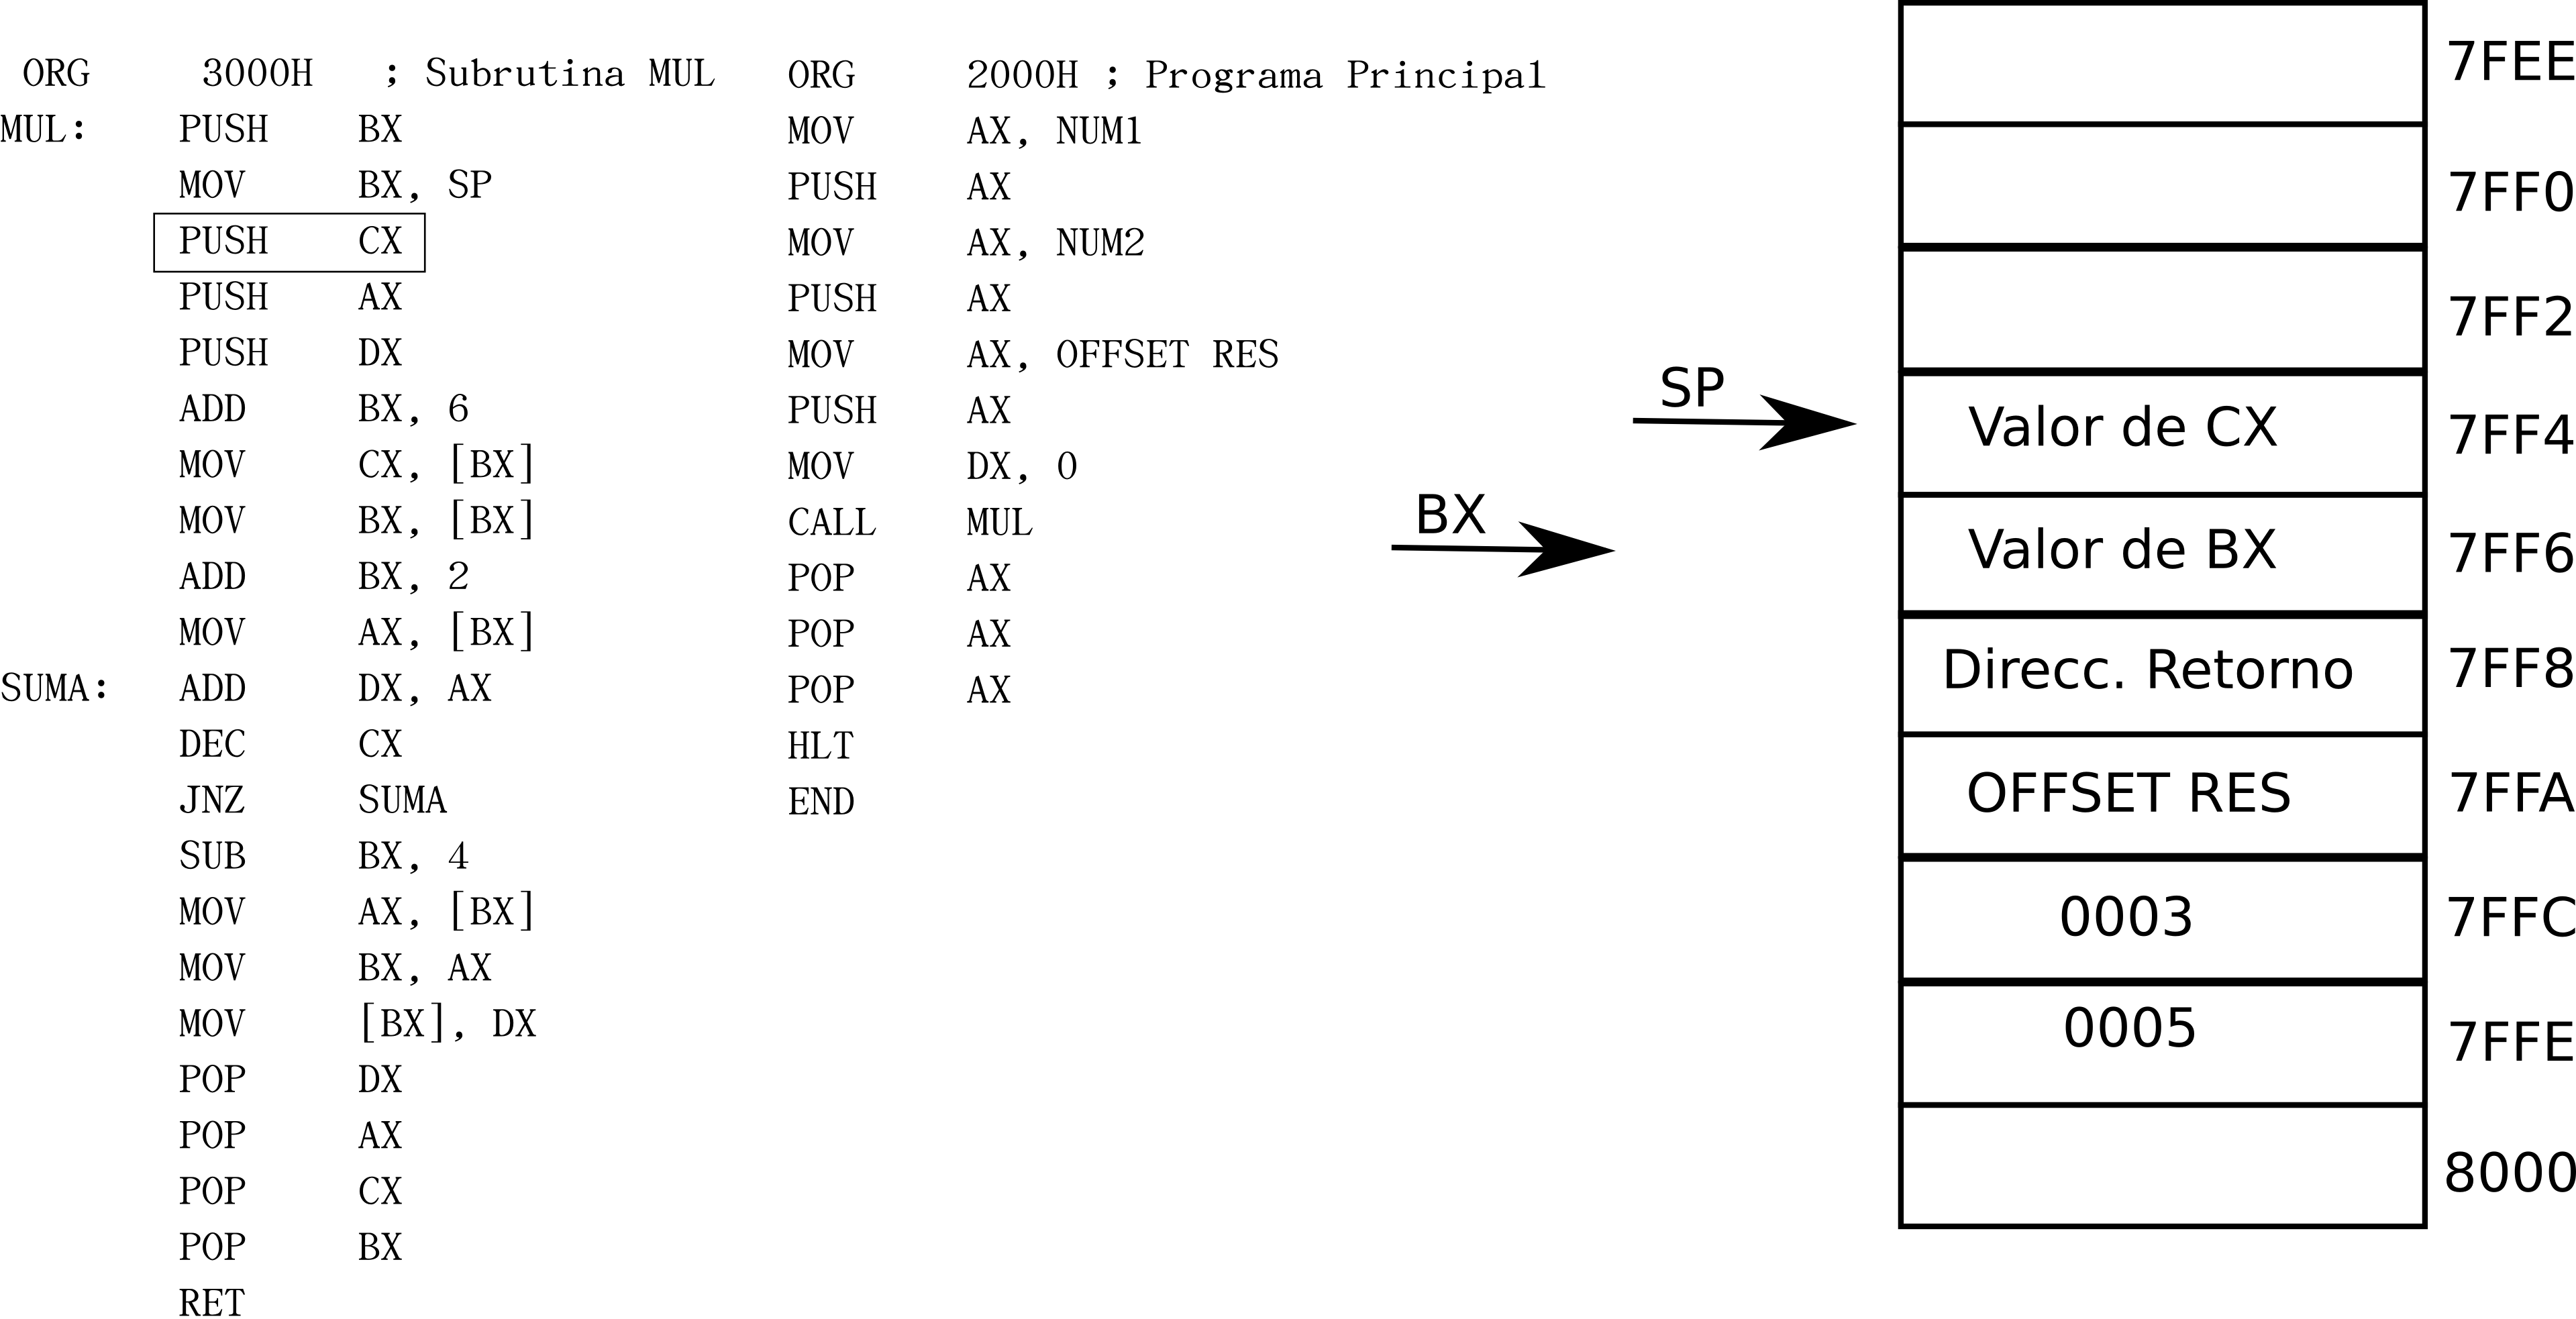
\includegraphics[scale=0.70]{imgs/imagen_008.png}
\end{frame}
\begin{frame}
  \frametitle{Ejercicio 7 - Pasaje de parámetros por pila}
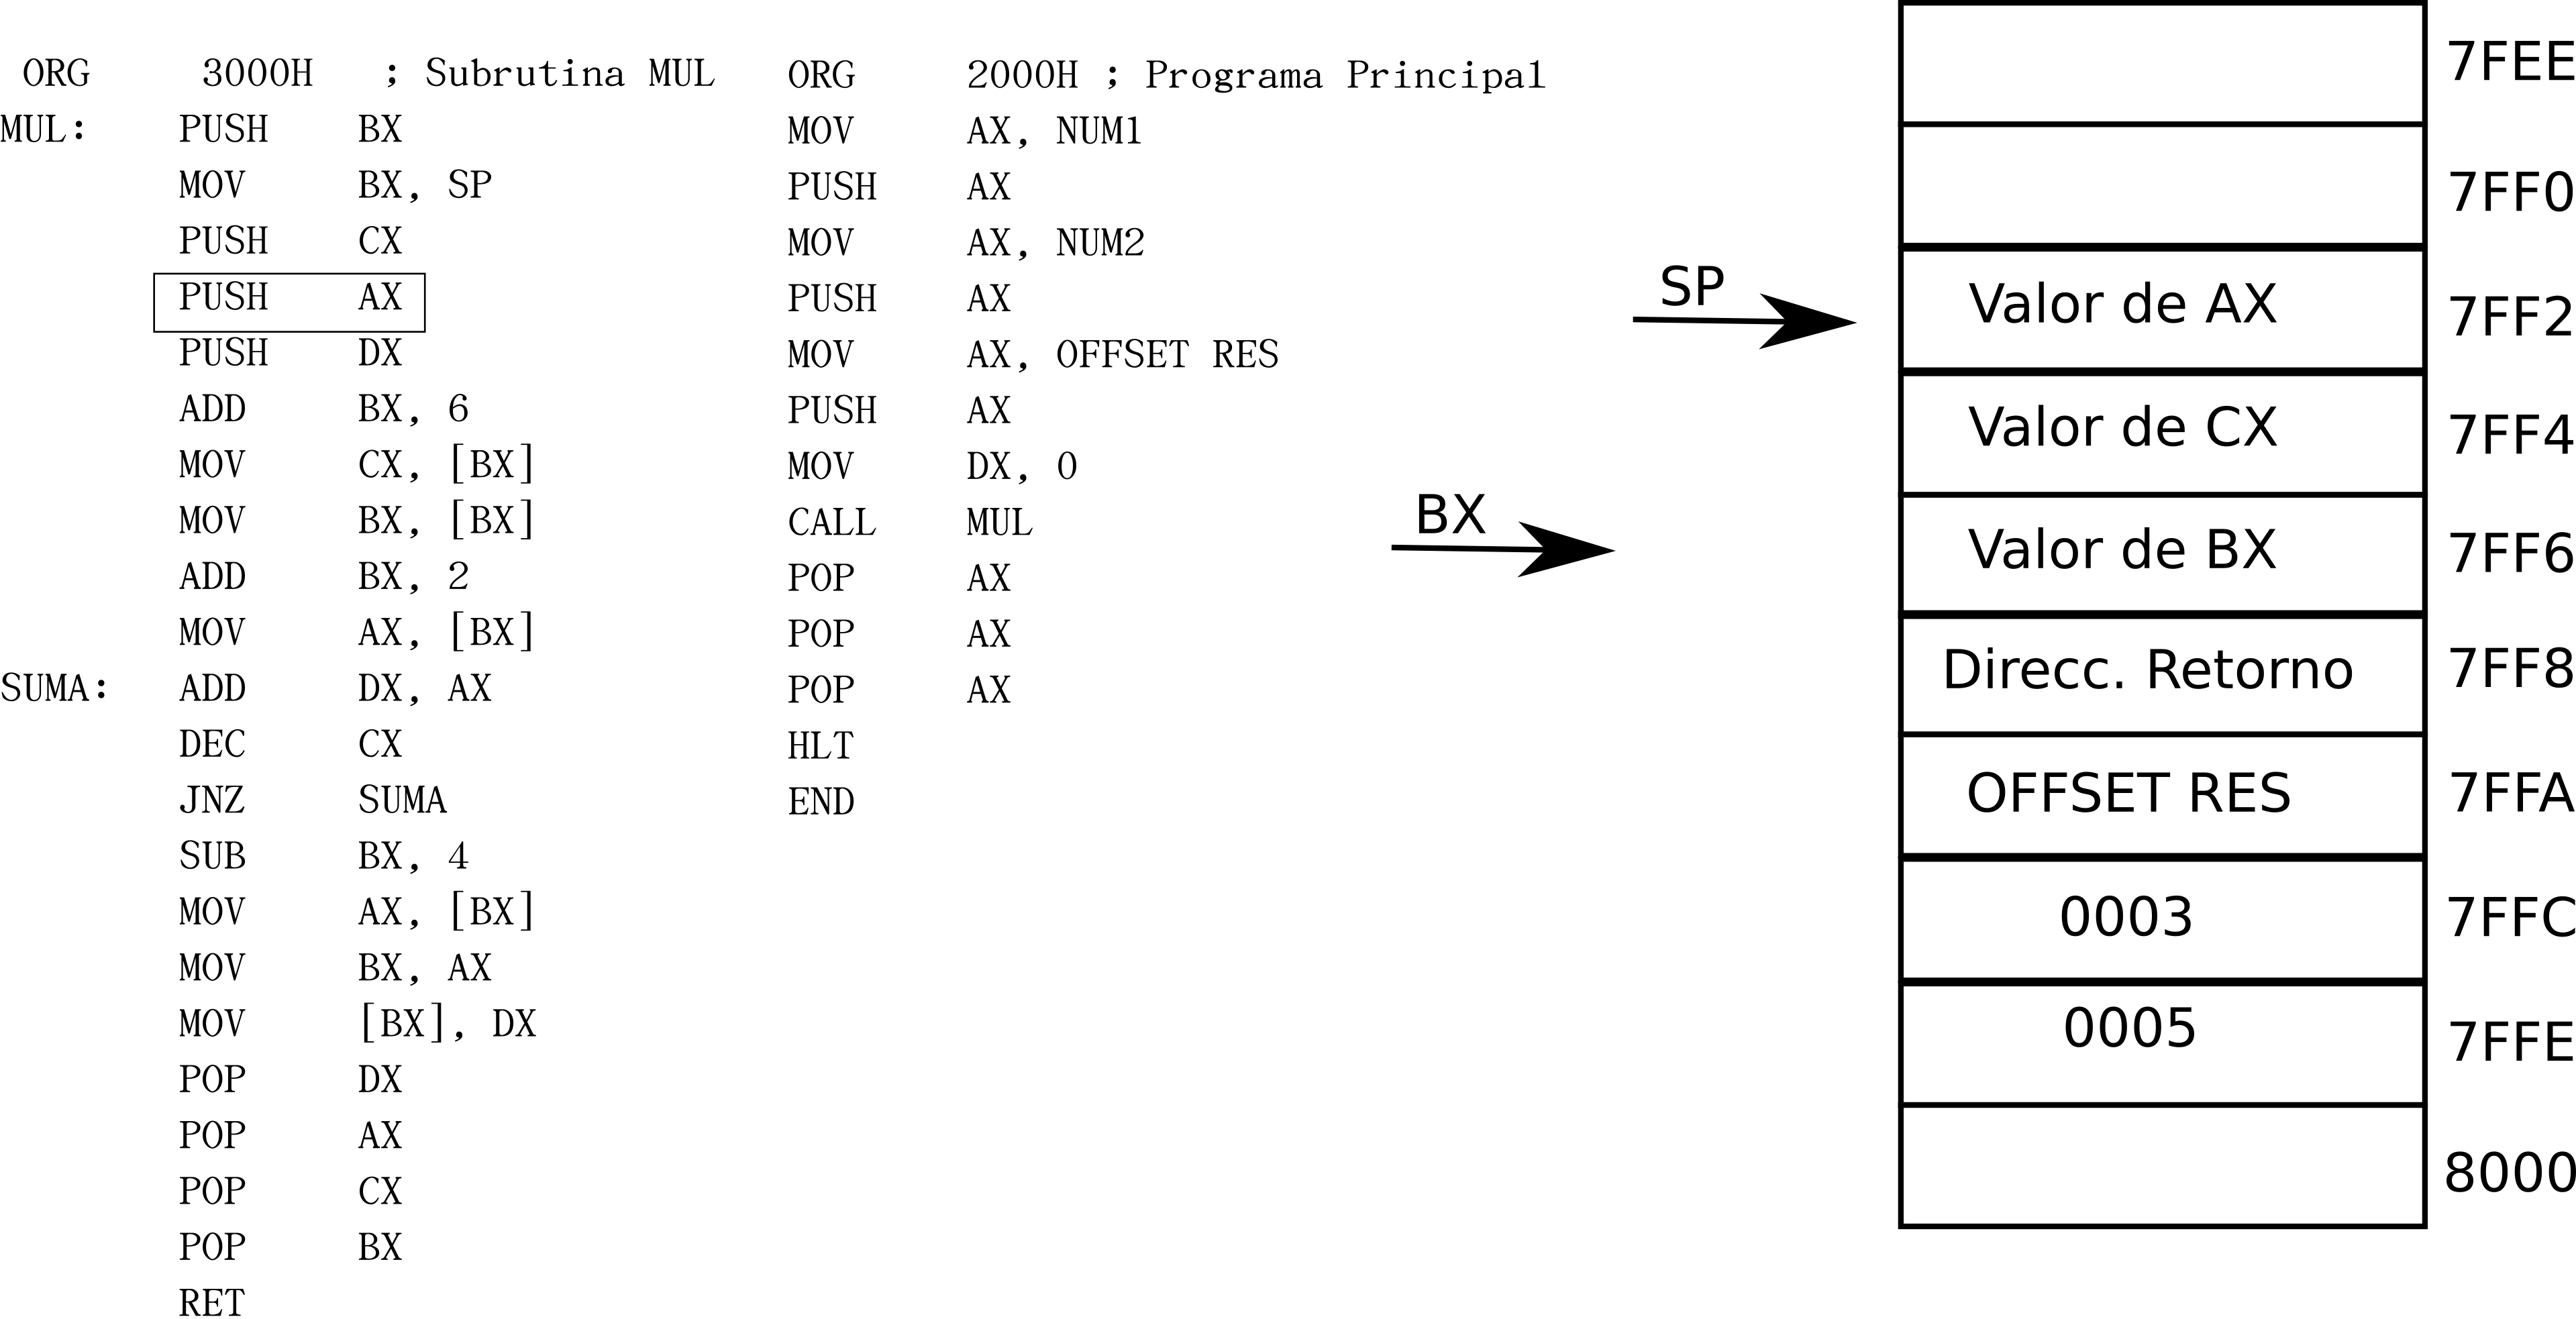
\includegraphics[scale=0.70]{imgs/imagen_009.png}
\end{frame}
\begin{frame}
\frametitle{Ejercicio 7 - Pasaje de parámetros por pila}
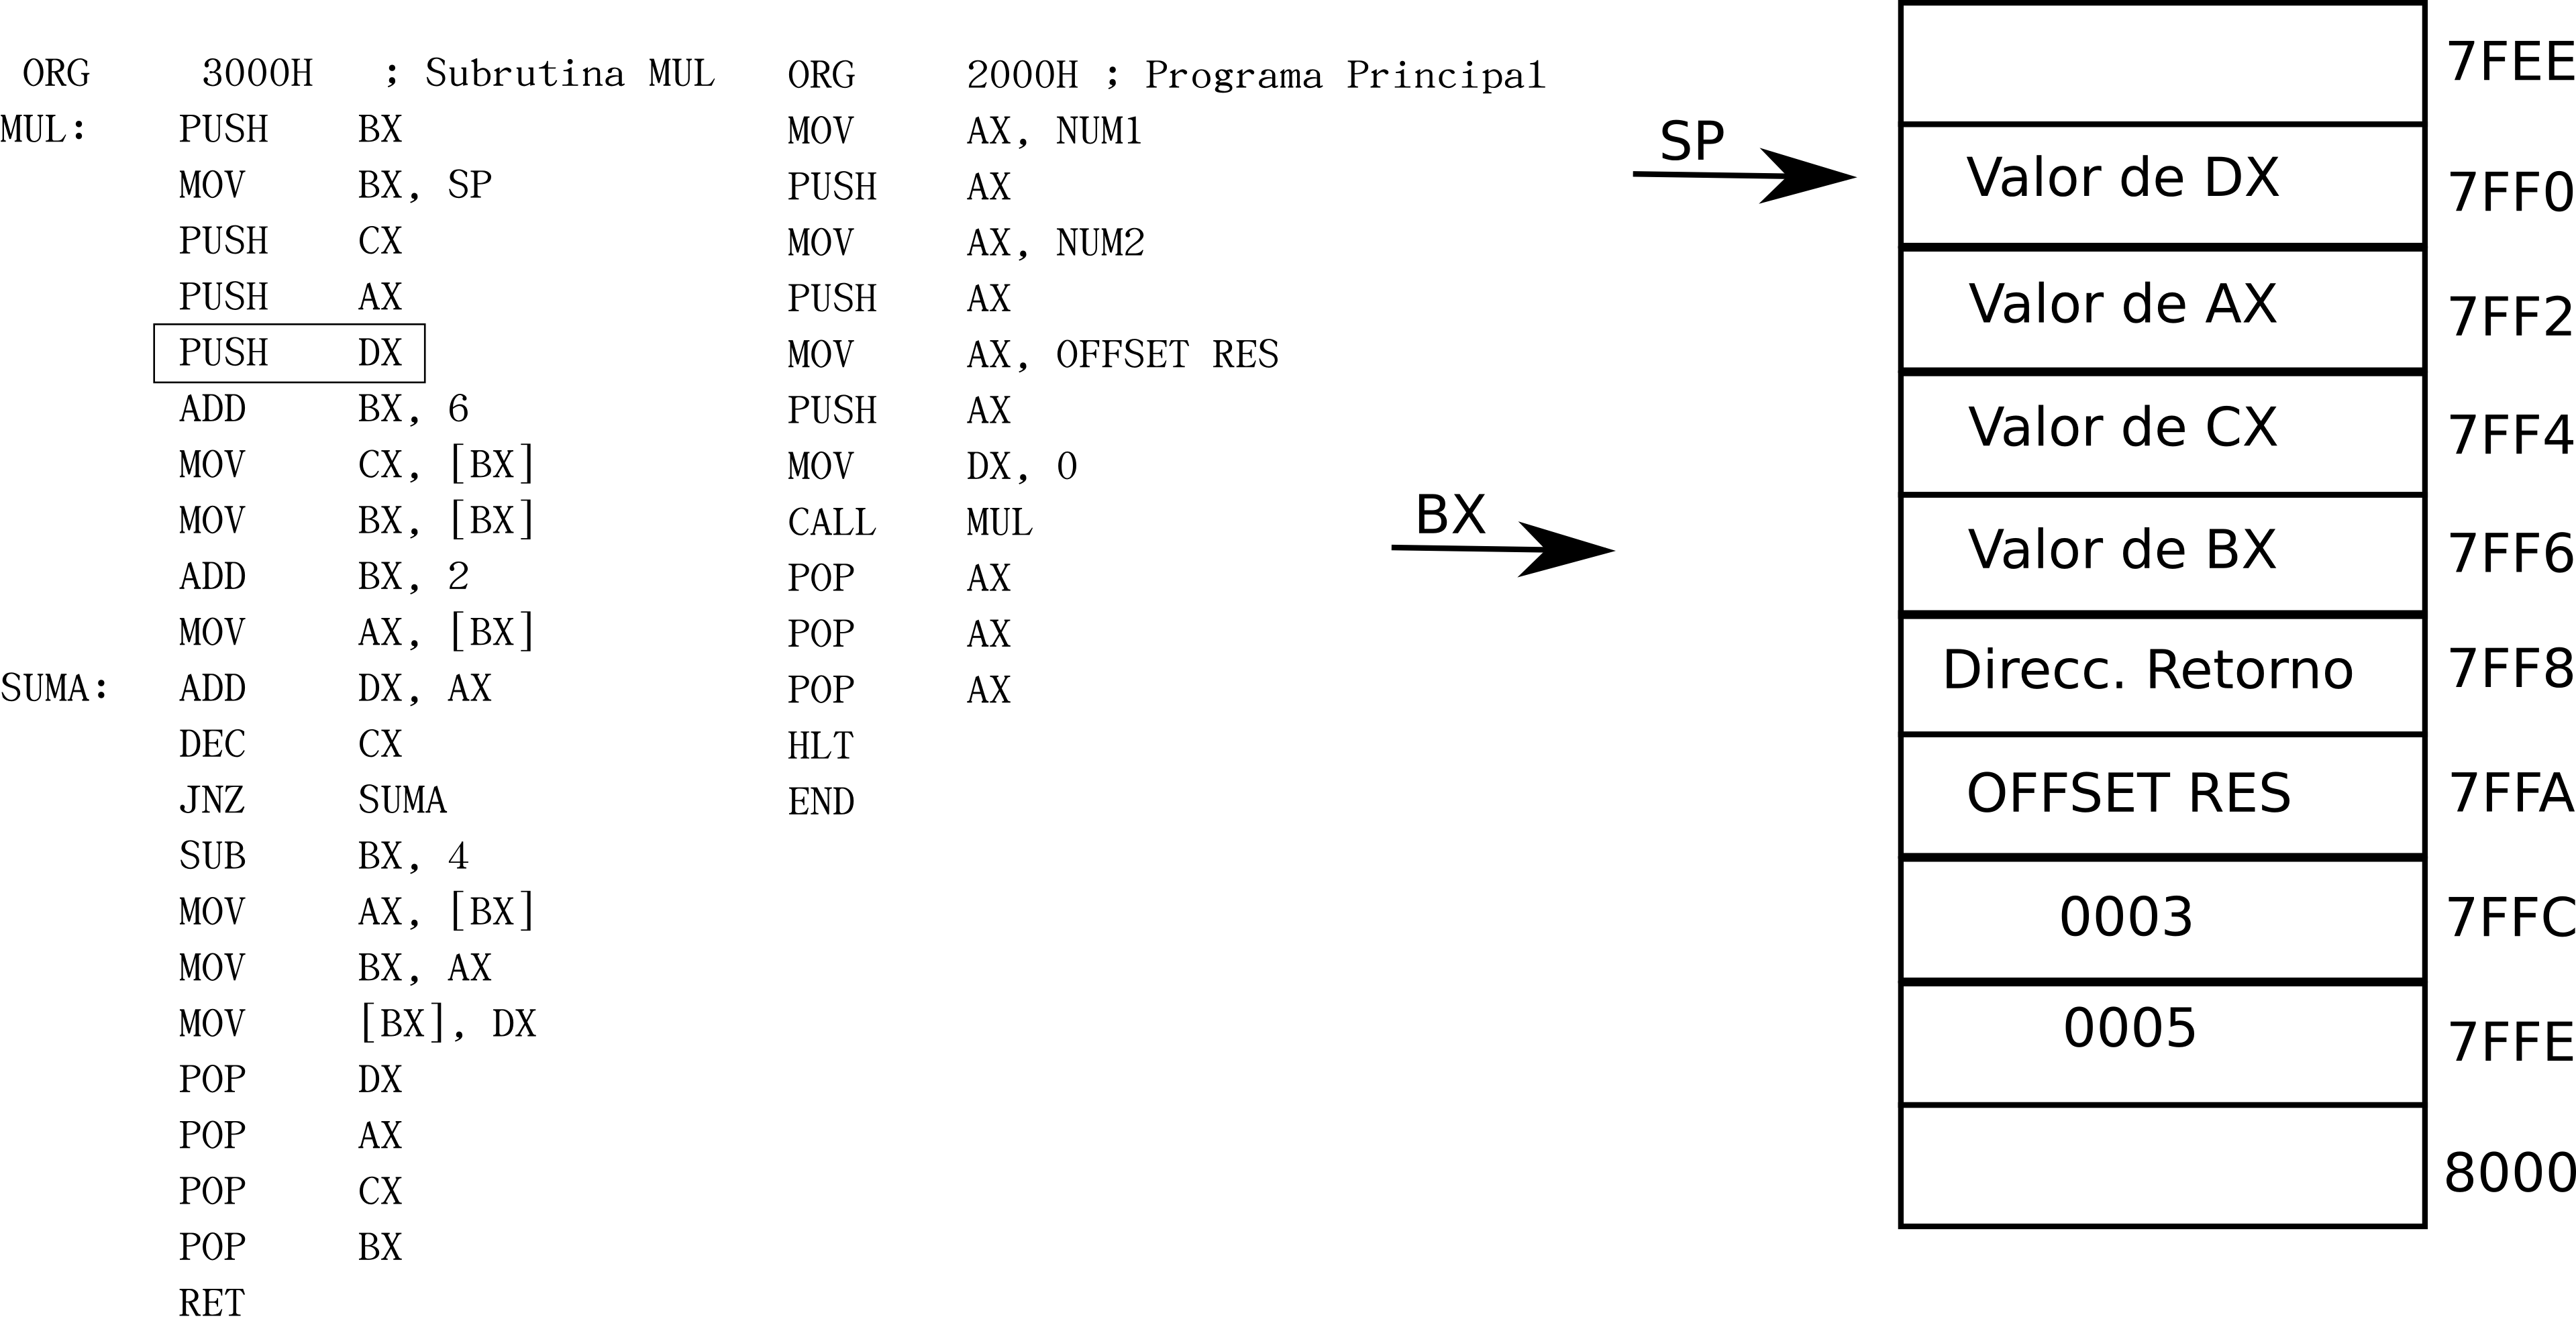
\includegraphics[scale=0.70]{imgs/imagen_010.png}
\end{frame}

\begin{frame}
\frametitle{Ejercicio 7 - Pasaje de parámetros por pila}
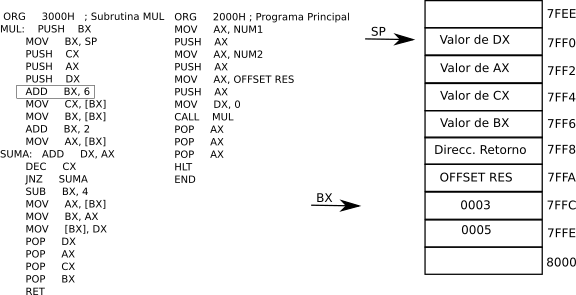
\includegraphics[scale=0.70]{imgs/imagen_011.png}
\end{frame}

\begin{frame}
\frametitle{Ejercicio 7 - Pasaje de parámetros por pila}
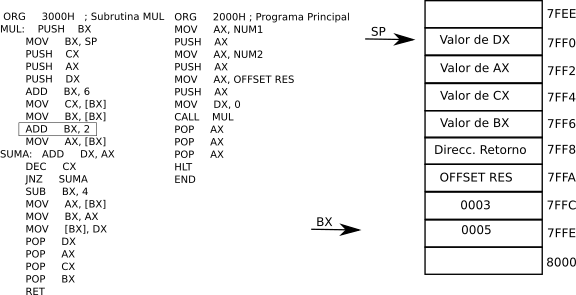
\includegraphics[scale=0.70]{imgs/imagen_012.png}
\end{frame}

\begin{frame}
\frametitle{Ejercicio 7 - Pasaje de parámetros por pila}
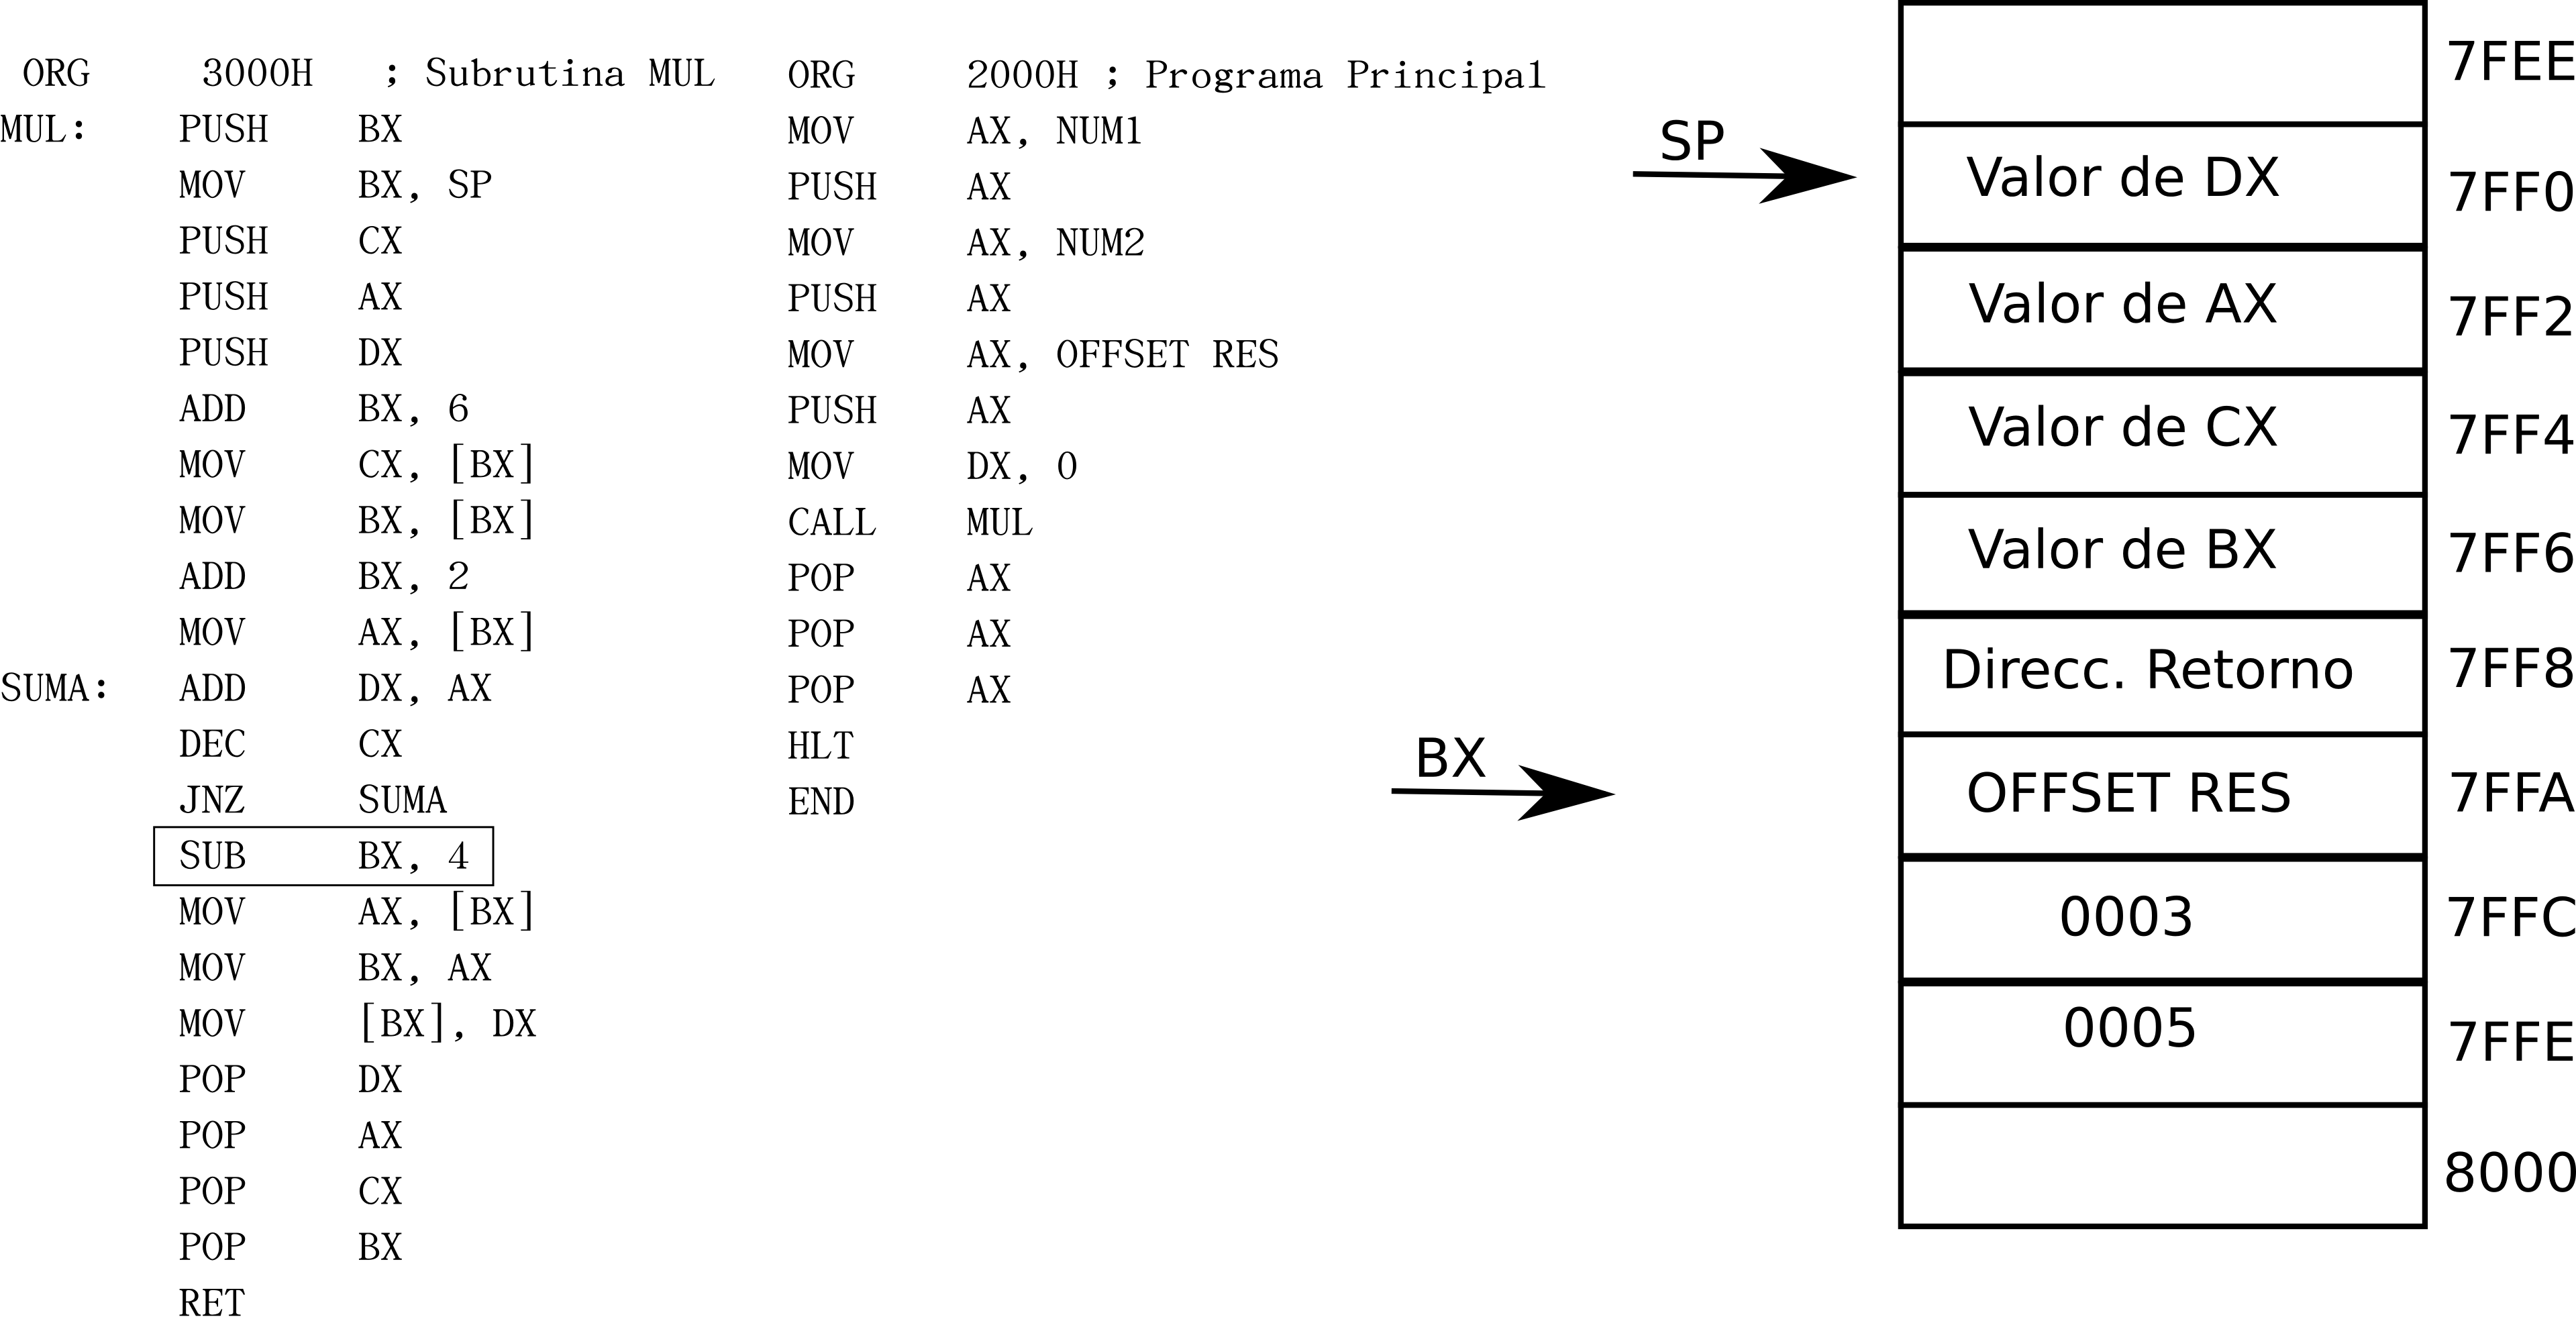
\includegraphics[scale=0.70]{imgs/imagen_013.png}
\end{frame}

\begin{frame}
\frametitle{Ejercicio 7 - Pasaje de parámetros por pila}
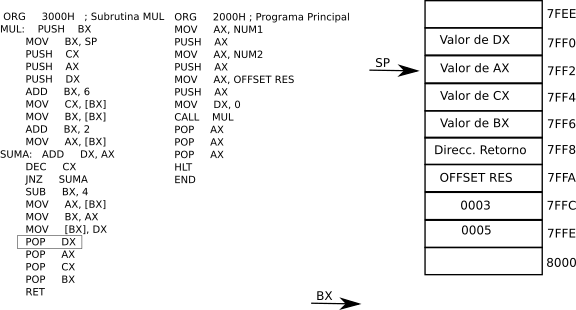
\includegraphics[scale=0.70]{imgs/imagen_014.png}
\end{frame}

\begin{frame}
\frametitle{Ejercicio 7 - Pasaje de parámetros por pila}
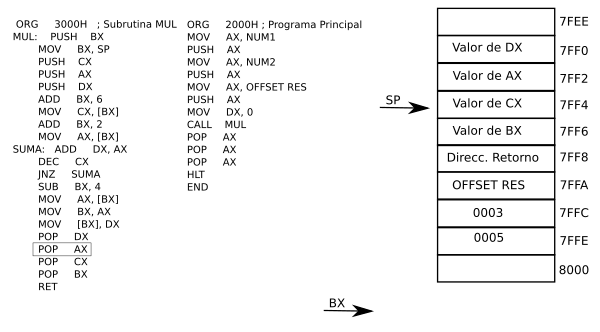
\includegraphics[scale=0.70]{imgs/imagen_015.png}
\end{frame}

\begin{frame}
\frametitle{Ejercicio 7 - Pasaje de parámetros por pila}
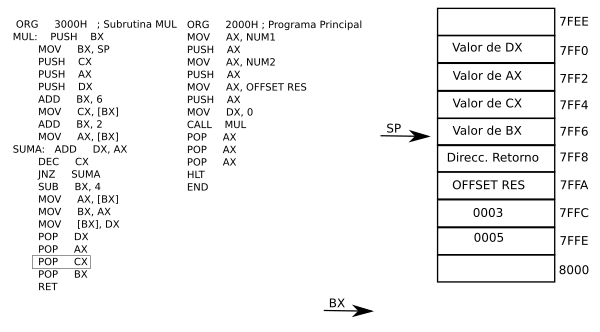
\includegraphics[scale=0.70]{imgs/imagen_016.png}
\end{frame}

\begin{frame}
\frametitle{Ejercicio 7 - Pasaje de parámetros por pila}
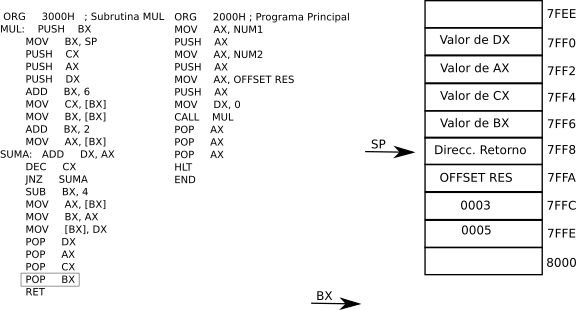
\includegraphics[scale=0.70]{imgs/imagen_017.png}
\end{frame}

\begin{frame}
\frametitle{Ejercicio 7 - Pasaje de parámetros por pila}
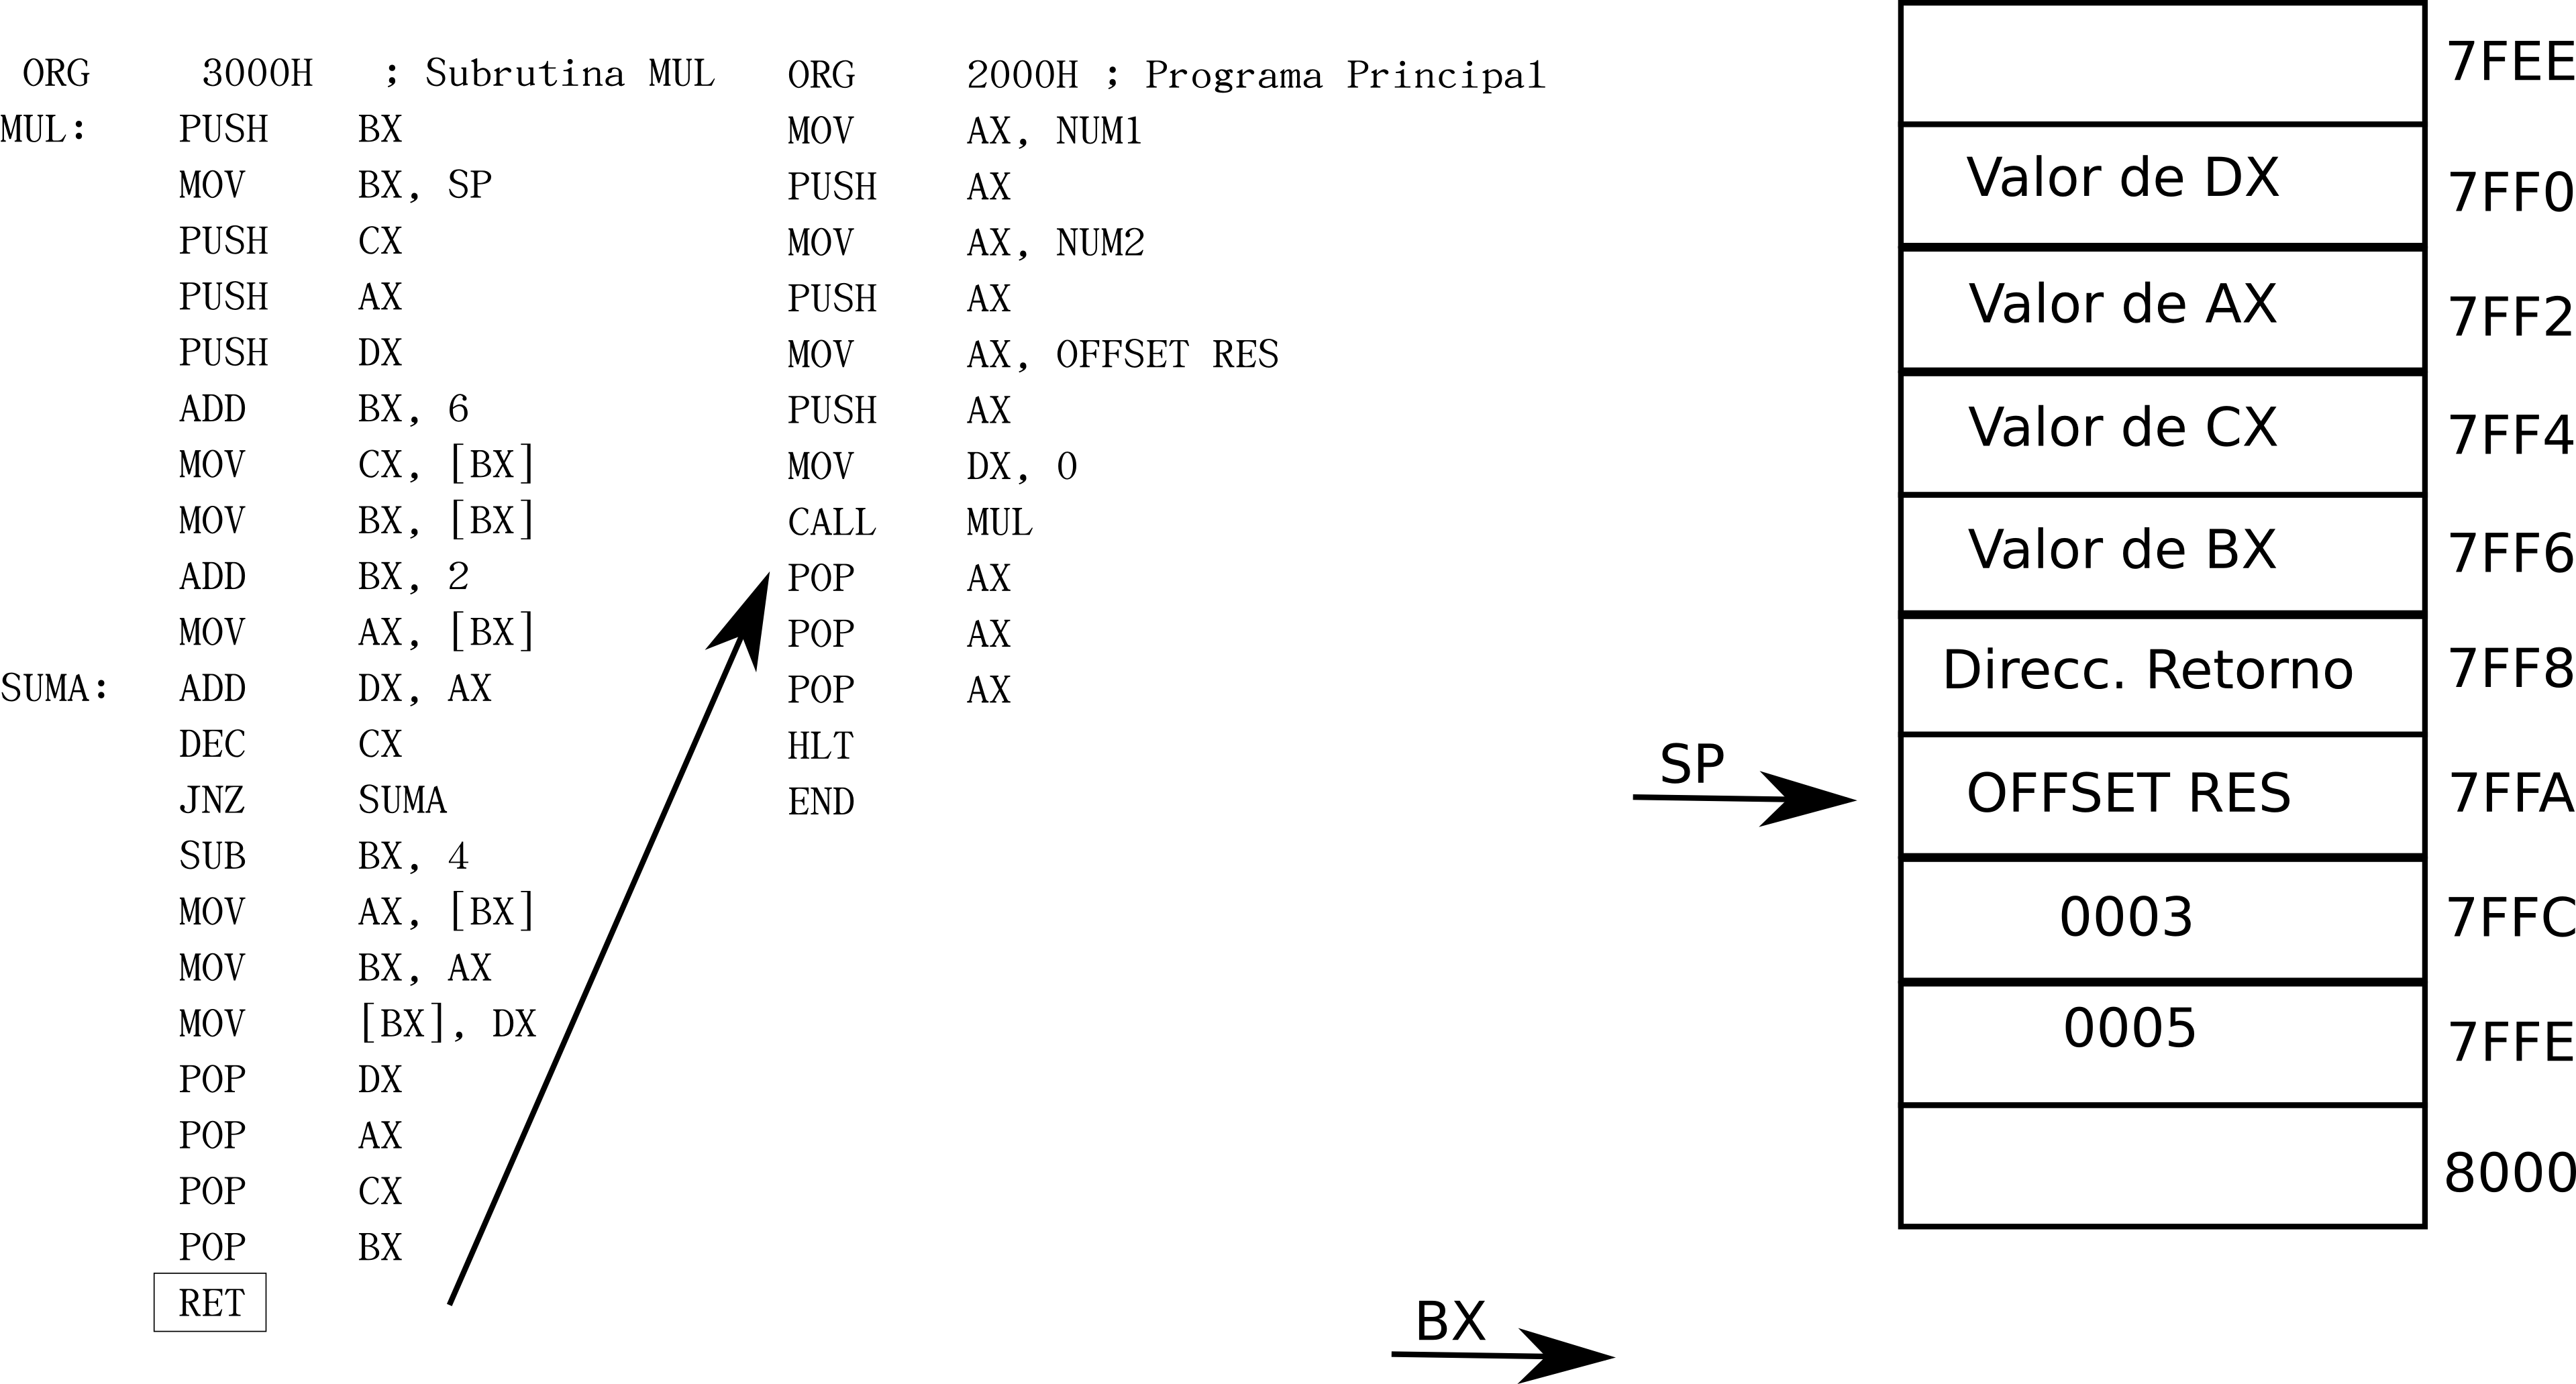
\includegraphics[scale=0.70]{imgs/imagen_018.png}
\end{frame}

\begin{frame}
\frametitle{Ejercicio 7 - Pasaje de parámetros por pila}
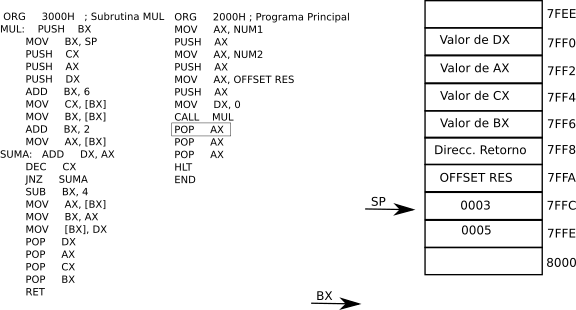
\includegraphics[scale=0.70]{imgs/imagen_019.png}
\end{frame}

\begin{frame}
\frametitle{Ejercicio 7 - Pasaje de parámetros por pila}
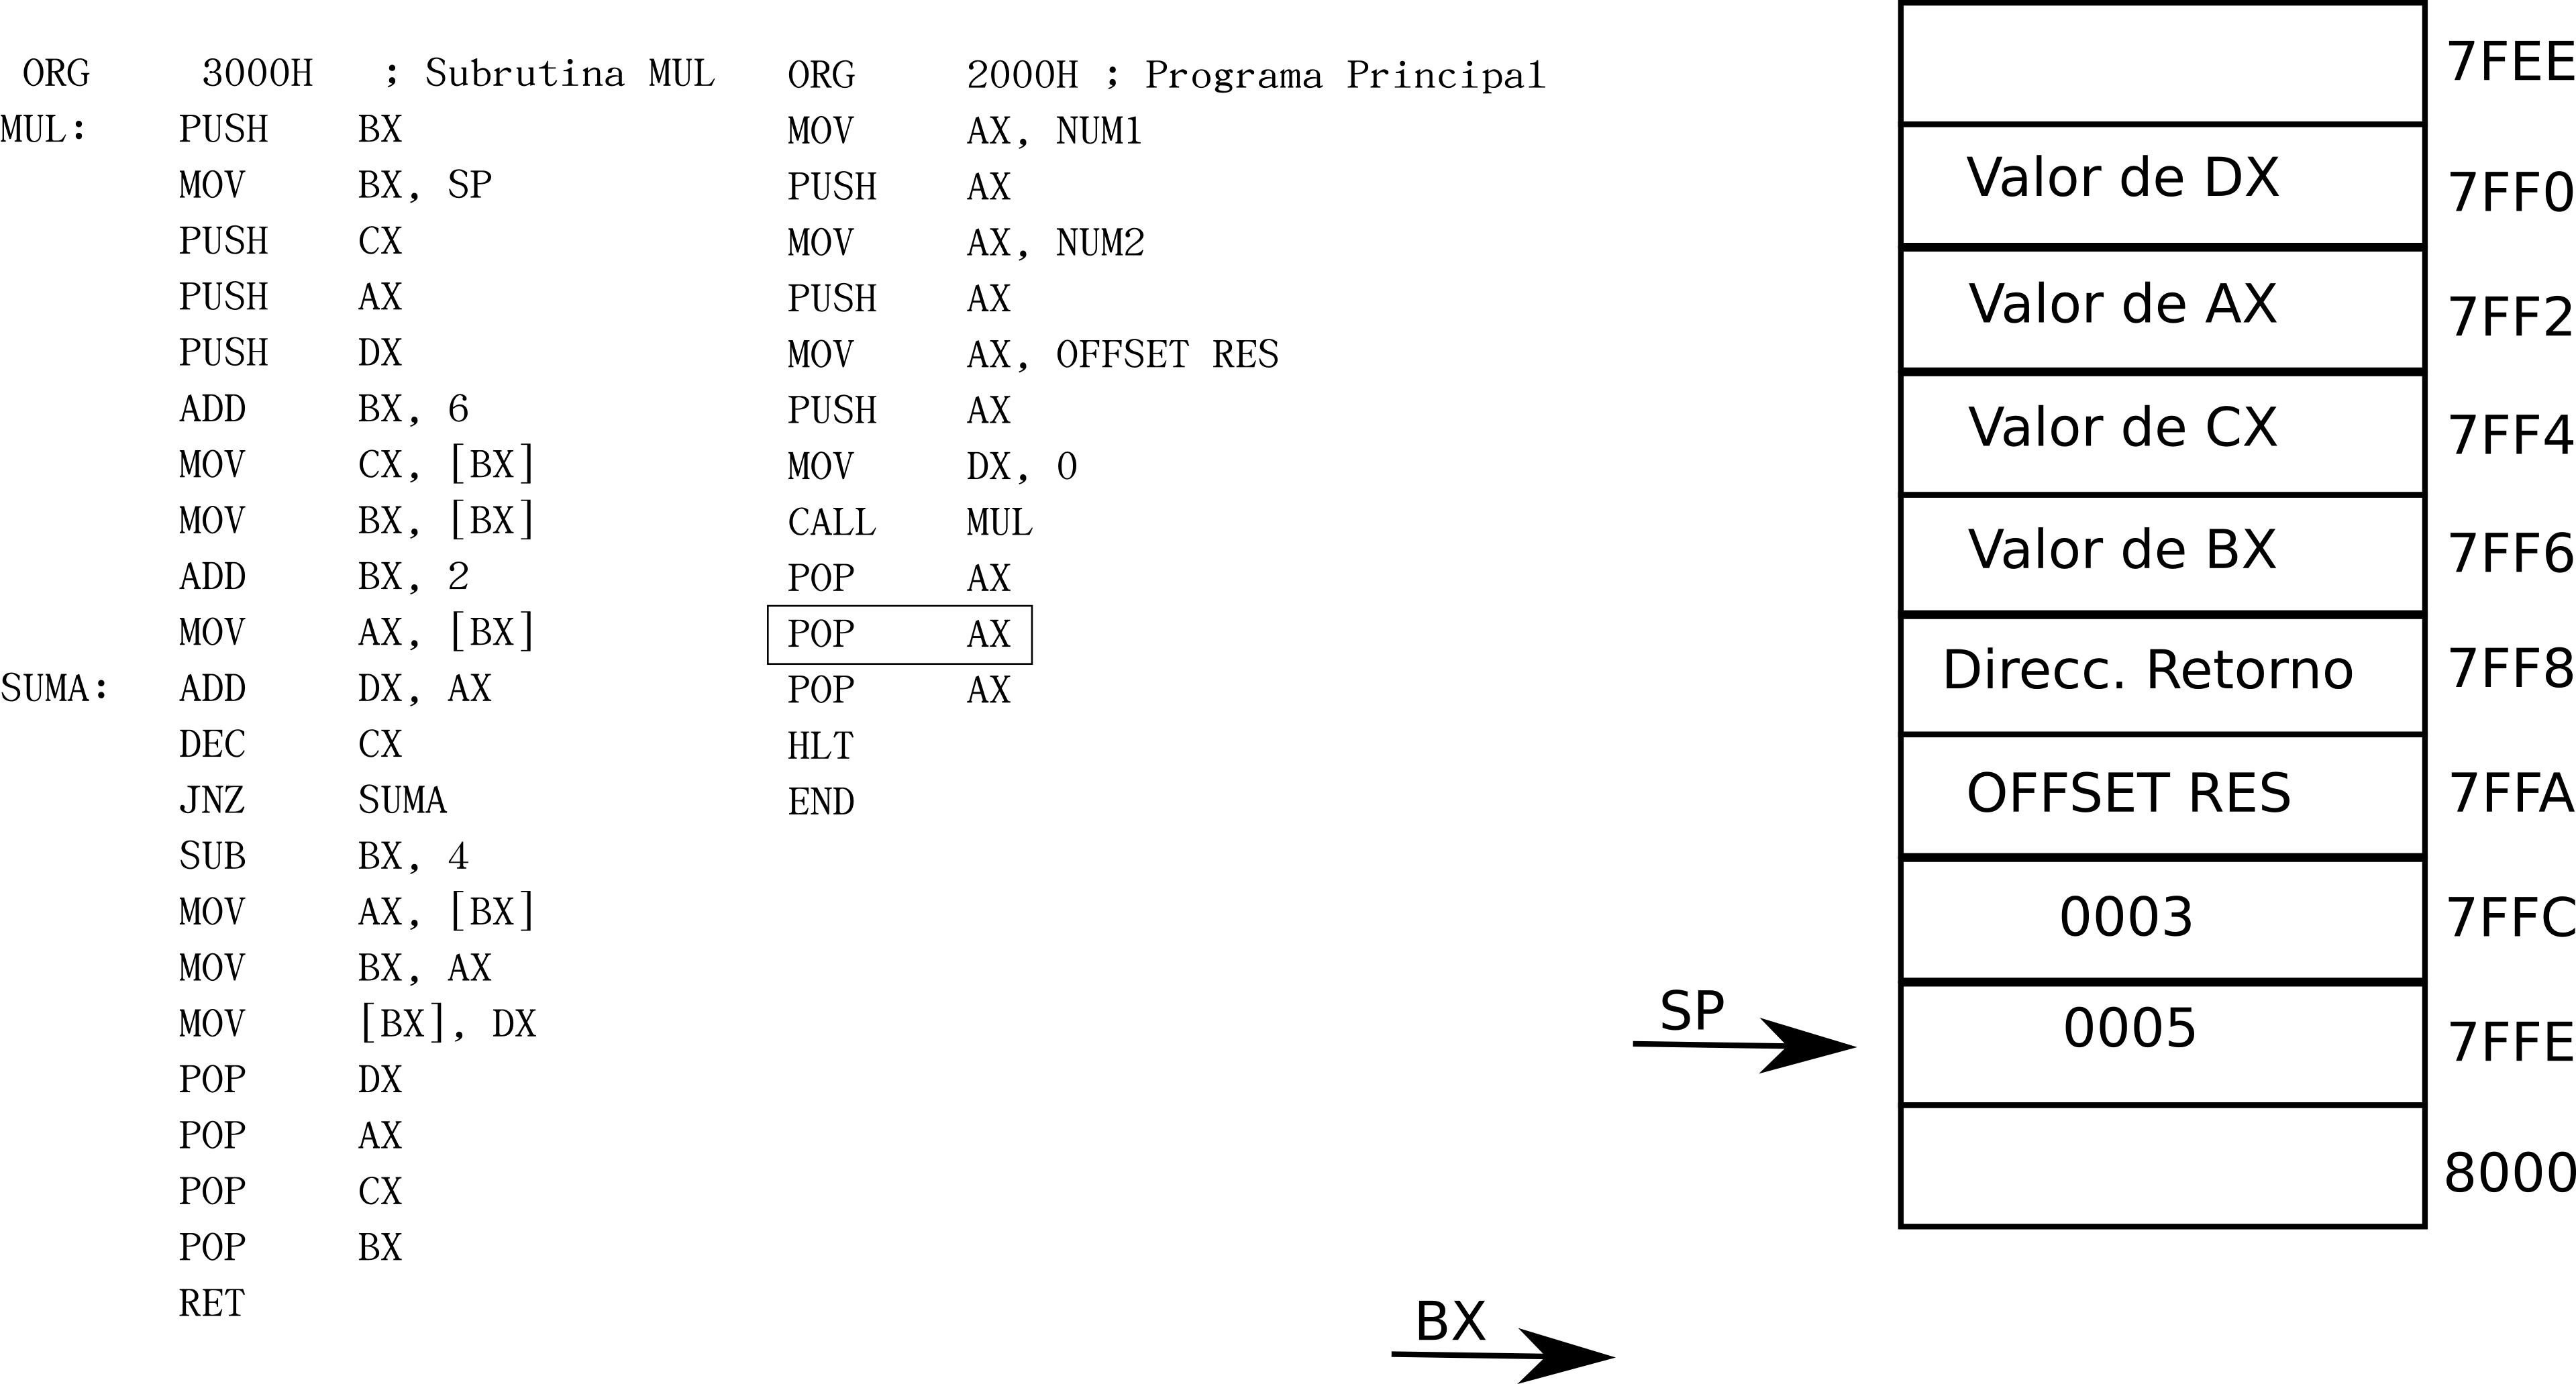
\includegraphics[scale=0.70]{imgs/imagen_020.png}
\end{frame}

\begin{frame}
\frametitle{Ejercicio 7 - Pasaje de parámetros por pila}
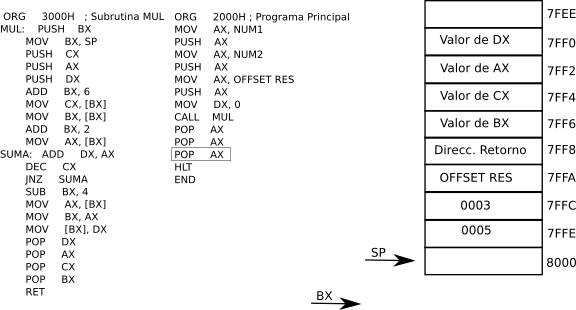
\includegraphics[scale=0.70]{imgs/imagen_021.png}
\end{frame}

\begin{frame}
\frametitle{Ejercicio 7 - Pasaje de parámetros por pila}
\includegraphics[scale=0.70]{imgs/imagen_022.png}
\end{frame}

\begin{frame}
\frametitle{Ejercicio 7 - Pasaje de parámetros por pila}
\includegraphics[scale=0.70]{imgs/imagen_023.png}
\end{frame}

\end{document}

